\documentclass{standalone}
\usepackage{mathpazo}
\usepackage{siunitx}
\usepackage[american voltages, american currents, american inductors]{circuitikz}
\newcommand*{\equal}{=}

\begin{document}
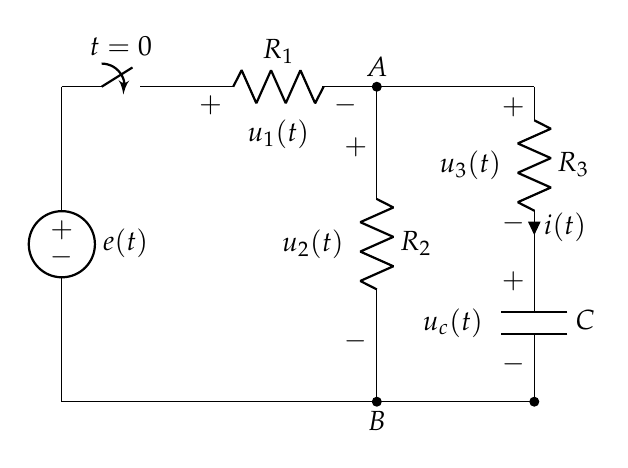
\begin{tikzpicture}
  \coordinate (A) at (0,4);
  \coordinate (B) at (4,4);
  \coordinate (C) at (6,4);
  \coordinate (D) at (0,0);
  \coordinate (E) at (4,0);
  \coordinate (F) at (6,0);
  \draw
  (A) to [closing switch, l = $t \equal 0$] ++(1.5,0)
  to [R, l = $R_1$, v = $u_1(t)$, -*] (B) node[above] {$A$}
  to [short] (C)
  (D) to [short, -*] (E) node[below] {$B$}
  to [short, -*] (F)
  (A) to [V, l = $e(t)$] (D)
  (B) to [R, l = $R_2$, v = $u_2(t)$] (E)
  (C) to [R, l = $R_3$, v = $u_3(t)$, i = $i(t)$] ++(0,-2)
  to [C, l = $C$, v = $u_c(t)$] (F);
  \end{tikzpicture}
\end{document}